\documentclass[a4paper,10pt]{article}

\usepackage[utf8]{inputenc}
%\usepackage[T1]{fontenc}
%\usepackage[french]{babel}
\usepackage[margin=1in]{geometry} 
\usepackage{amsmath,amsthm,amssymb}
\usepackage{lmodern}
\usepackage{graphicx}
\usepackage{mathtools}
\usepackage{tcolorbox}
\usepackage{listings}
\usepackage{subcaption} % pour le subplot

\newcommand{\R}{\mathbb{R}}  
\newcommand{\Z}{\mathbb{Z}}
\newcommand{\N}{\mathbb{N}}
\newcommand{\Q}{\mathbb{Q}}
\newcommand{\C}{\mathbb{C}}
\DeclareMathOperator*{\argmax}{arg\,max}
\DeclareMathOperator*{\argmin}{arg\,min}
%opening
\title{Intership - Sparse Coding and w learning}
\author{Thomas Rolland}
\date{}%Remove date

\begin{document}

\maketitle

\begin{abstract}
Little document to summarize state-of-the-art sparse coding and dictionary learning for weekly supervised  and unsupervised  feature extraction in speech. Introduction to 1.2 are  based on the Hugo Larochelle courses.\\
\begin{center}

\textbf{This document is a draft }
 
\end{center}
\end{abstract}
\tableofcontents
%\section{Pré-requis}
%\subsection{Representation learning}
%La Representation learning ou feature learning sont des méthodes qui permettent à un système
\section{Sparse coding}
\subsection{Introduction}
\paragraph{Idea} Sparse dictionary learning is a representation learning method which aims at finding a sparse representation of the input data (in form of a linear combination of basic elements (called Atoms). The idea of using learned dictionary instead of a predefined one is based on wavelets. The sparse learned models has recently led to state-of-the-art result for denoising, classification,...
%UNSPERVISED LEARNING=========================================================+
\paragraph{Unsupervised learning} Only use the inputs $x^{(t)}$ ( $X = [x_1,....,x_n]$ in $\R^{m \times n}$) for learning. Automatically extract meaningful features of our data, leverage the availability of unlabeled data and add a data-dependent regularize to trainings.\\

Sparse coding is one of the neural networks used for unsupervised learning  (like restricted boltzmann machines and autoencoders).\\
The idea behind sparse coding is: For each $x^{t}$ find a latent representation $h^{t}$ such that:
\begin{itemize}
 \item[$\bullet$] It is sparese: the vector $h^{t}$ has many zeros (only few nonzero elements)
 \item[$\bullet$] We can reconstruct the original input $x^{(t)}$ as well as possible.
\end{itemize}
That mean, more formally:\\

%Formulation du problème=============================
\begin{center}
 $\min\limits_{D} \frac{1}{T} \sum_{t=1}^{T}  \min\limits_{h^{(t)}} \frac{1}{2} \| x^{(t)} - D \hspace{3px} h^{(t)} \|_2^2 + \lambda \|h^{(t)} \|_1$\\
\end{center}

 %Explicaiton de la formulation=========================
 \begin{itemize}
 \item[$\bullet$] D is a matrix of weights, usually refer to that matrix as a dictionary matrix (containt atoms) with $D \in  \R^{m \times k}$ ( k the number of atoms)
  \item[$\bullet$] $\| x^{(t)} - D \hspace{3px} h^{(t)} \|_2^2 $ is the reconstruction error
  \item[$\bullet$]$ D \hspace{3px} h^{(t)}$ is the reconstruction of $\hat{x}^{(t)}$
  \item[$\bullet$]$\|h^{(t)} \|_1$ is the sparsity penalty (more 0 in h we have, better it is)
 \end{itemize}
This two objectives fight each other. But it still a optimization problem (cf min), and we'll try to optimize it for each training example $x^{(t)}$. This is why we have a sum over all the training examples.
\newline

%Contraintes sur D======================================
\indent We also constrain the columns of D to be of norm 1 (otherwise, D could grow big while $h^{(t)}$ becomes small to satisfy the prior). And sometimes the columns are constrained to be no greather than 1.\\

However, $h^{(t)}$ is now a complicated function of $x^{(t)}$:\\
Encoder is the minimization $h(x^{(t)}) = arg\min\limits_{h^{(t)}}= \frac{1}{2} \| x^{(t)} - D \hspace{3px} h^{(t)} \|_2^2 + \lambda \|h^{(t)} \|_1$, so the optimization problem is more complicated than a simple non linear problem.\\
The idea to solve this minimization problem is \cite{NIPS2006_2979}

\begin{lstlisting}[language=Python,frame=single]
while D not_converged :
    Fix D
    Minimize h           (1) // Sparse Coding step
    Fix h 
    Minimize D           (2) // Update Dictionary step
\end{lstlisting}

But there are some improvement like K-SVD algorithm \cite{KSVD}, which compute column by column a SVD computation over the relevant examples.
%DICTIONARY==================================================================+  
\paragraph{Dictionary}
We can also write $\hat{x}^{(t)} = D\hspace{3px} h(x^{(t)}) \displaystyle\sum_{\substack{k s.t.\\ h(x^{(t)})_k\neq 0}}  D.,_k h(x^{(t)} )_k$
\begin{figure}[h]
 \centering
 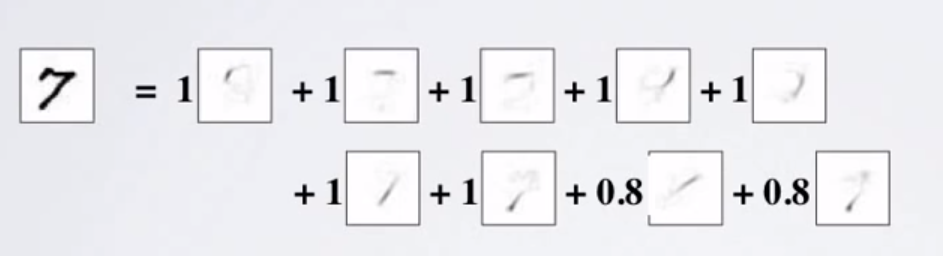
\includegraphics[scale=0.5]{spacecoding_1.png}
 % spacecoding_1.png: 943x256 px, 96dpi, 24.95x6.77 cm, bb=0 0 707 192
  \caption{Example of reconstruction using sparse coding}
\end{figure}

The images refer to $D.,_k$ (columns of D wich are not equals to 0) and the factor (1 or 0.8 in this case) refer to $h(x^{(t)} )_k$
\\We also refer to D as the dictionary:
\begin{itemize}
 \item[$\bullet$]in certain applications, we know what dictionary matrix to use
 \item[$\bullet$]often however, we have to learn it
\end{itemize}

In general we have $k<<n$ . But we can use an overcomplete dictionary with $k > m$.
\subsection{Inderence of Sparse code}
The orginal problem is a combinatorial problem (proven to be NP-hard). To solve this problem we use relaxation methods (then we can smooth the $L_0$ and use continious optimization techniques) or greedy methos (then build the solution one non-zero element at time).
\subsubsection{Compute h }
%Inderence of sparse code=============================================
\paragraph{Idea}
Here we develop  step (1) of our algorithm.\\
Assume we are given a dictionary matrix D, how do we compute $h(x^{(t)})$. We have to optimize:
\begin{center}  Basic Pursuit:
$l(x^{(t)}) = \frac{1}{2} \| x^{t}- D h^{(t)} \|^{2}_{2} + \lambda \|h^{(t)}\|_1 w.r.t. h^{(t)}$\\ 
\end{center} 
Here we used relaxation method to switch from norm $l_0$ to $l_1$ know as the  Basic Pursuit (vs Matching Pursuit,a greedy method,  if we keep $l_0$ norm and find one atom at a time).\\
We could use a gradient descent method to solve this minimization:\\
\begin{center}
$\Delta_{h^{(t)}} l(x^{(t)}) = D^T (D h^{(t)} - x^{(t)}) + \lambda sign(h^{(t)})$
\end{center}
The issue is $l_1$ norm is not differentiable at 0. The solution is : if $h^{(t)}$ changes sign because of $l_1$ norm gradient then clamp to 0.That mean :

$h^{(t)}_k = h^{(t)}_k   - \alpha (D_{., k})^T (D h^{(t)} - x^{(t)})$\\
\indent if  sign($h^{(t)}_k) \neq$ sign$(h^{(t)}_k - \alpha \lambda$ sign$(h^{(t)}_k) )$ then: $h^{(t)}_k = 0$\\
\indent else $h^{(t)}_k = h^{(t)}_k - \alpha \lambda$ sign$(h^{(t)}_k)$
\paragraph{ISTA (Iterative Shrinkage and Thresholding Algorithm)}
:
\begin{lstlisting}[language=Python,frame=single]
initialize h 
while h not_converged:
    for each h_k in h:
        h_k = h_k -alpha * transpose(D[:,k]) * (D*h - x)
        h_k = shrink(h_k,alpha*lambda_coef)
return h
\end{lstlisting}
Here \textbf{shrink(a,b) }= [..., sign$(a_i)$ max($|a_i| - b_i$, 0), ...]\\

\subsubsection{Compute D}
There are three algorithms used for  dictionary update.
\paragraph{Algorithm 1: A gradient descent method}
Our original problem is:
\begin{center}
 $\min\limits_{D} \frac{1}{T} \sum_{t=1}^{T}  \min\limits_{h^{(t)}} \frac{1}{2} \| x^{(t)} - D \hspace{3px} h^{(t)} \|_2^2 + \lambda \|h^{(t)} \|_1$\\
\end{center}
But here we assume $h(x^{(t)})$ doesn't depend on D. So we must minimize:
\begin{center}
 $\min\limits_{D} \frac{1}{T} \sum_{t=1}^{T}  \min\limits_{h^{(t)}} \frac{1}{2} \| x^{(t)} - D \hspace{3px} h^{(t)} \|_2^2 $\\
\end{center}
\begin{lstlisting}[language=Python,frame=single]
while D not_converged:
    # Perform gradient update of D
    D = D - alpha * (1/T)* sum((x - D h)* tranpose(h))
    # Renormalize the columns of D
    for each column D[:,j]:
        D[:,j] = (D[:,j] / norm(D[:,j]))

return D
\end{lstlisting}

\paragraph{Algorithm 2: Block-coordinate descent}
We must minimize:
\begin{center}
 $\min\limits_{D} \frac{1}{T} \sum_{t=1}^{T}  \min\limits_{h^{(t)}} \frac{1}{2} \| x^{(t)} - D \hspace{3px} h^{(t)} \|_2^2 $\\
\end{center}
The idea is to solve for each column $D_{., j}$ in cycle (that mean to optimize in one direction at time). For that we must set the gradient for $D_{., j}$ to zero.\\
We have:
\begin{center}
 $0 = \frac{1}{T}\sum_{t=1}^{T} (x^{(t)} - D h(x^{(t)}))$ $h^{(t)}_{j}$\\ \vspace{0.4cm}
 We separe $D_{.,j}$ from the rest of D:\\
 $0 = \frac{1}{T}\sum_{t=1}^{T} (x^{(t)} - (\sum_{i \neq j}D_{.,i}$ $h(x^{(t)})_i$ $ )$  $ - (D_{.,j}$ $h(x^{(t)})_j)$ ) $ h^{(t)}_{j}$\\ \vspace{0.4cm}
 Our aim is to find the value of $D_{.,j}$, we must isolate $D_{.,j}$ :\\
 $0 = \frac{1}{T} \sum_{t=1}^{T}(x^{(t)} h^{(t)}_{j} - (\sum_{i \neq j}D_{.,i}$ $h^{(t)}_i$ $h^{t}_{j} )$  $ - (D_{.,j}$ $h^{(t)2}_j))$\\ \vspace{0.2cm}
 
  $0 = (\sum_{t=1}^{T}(x^{(t)} h^{(t)}_{j} - (\sum_{i \neq j}D_{.,i}$ $h^{(t)}_i$ $h^{t}_{j} )$  $) - ( \sum_{t=1}^{T}( D_{.,j}$ $h^{(t)2}_j)))$\\ \vspace{0.2cm}
  
  $  \sum_{t=1}^{T}( D_{.,j}$ $h^{(t)2}_j) = \sum_{t=1}^{T}(x^{(t)} h^{(t)}_{j} - (\sum_{i \neq j}D_{.,i}$ $h^{(t)}_i$ $h^{t}_{j} )$  $) $\\  \vspace{0.2cm}
  
  $ D_{.,j}  \sum_{t=1}^{T} h^{(t)2}_j = \sum_{t=1}^{T}(x^{(t)} h^{(t)}_{j} - (\sum_{i \neq j}D_{.,i}$ $h^{(t)}_i$ $h^{t}_{j} )$  $) $\\ \vspace{0.2cm}
  
$ D_{.,j}  =\frac{1}{ \sum_{t=1}^{T} h^{(t)2}_j} \sum_{t=1}^{T}(x^{(t)} h^{(t)}_{j} - (\sum_{i \neq j}D_{.,i}$ $h^{(t)}_i$ $h^{t}_{j} )$  $) $\\ \vspace{0.2cm}

$ D_{.,j}  =\underbrace{\frac{1}{ \sum_{t=1}^{T} h^{(t)2}_j}}_{A_{j, j}} \underbrace{\sum_{t=1}^{T}(x^{(t)} h^{(t)}_{j})}_{B_{., j}}  - \sum_{i \neq j}D_{., i}($ $\underbrace{\sum_{t=1}^{T} h^{(t)}_i h^{t}_{j} ) }_{A_{i,j}}$\\ \vspace{0.2cm}
$D_{., j} = \frac{1}{A_{j, j}}(B_{., j} - D A_{., j} + D_{., j}A_{j, j})$
\end{center}  
\begin{lstlisting}[language=Python,frame=single]
while D not_converged:
    # For each column D[:,j] perform updates
    for each column D[:,j]:
        D[:,j] = (1/A[j, j])*(B[:, j] - D A[:, j] + D[:, j] A[j, j])
        # Normalization
        D[:,j] = D[:,j]/norm(D[:,j])

return D
\end{lstlisting}

\paragraph{Algorithm 3:  Online learning algorithm}
For large datasets we want to update D after  visiting each $x^{(t)}$. The solution is for each $x^{(t)}$ \cite{Mairal:2009:ODL:1553374.1553463} :
\begin{itemize}
 \item[$\bullet$]  Perform inference of $h(x^{(t)})$ after visiting each $x^{(t)}$
 \item[$\bullet$]  Update running averages of the quantities required to update D: 
        \begin{itemize}
         \item B = $\beta B + (1 - \beta) x^{(t)}h(x^{(t)})^T$
         \item A = $\beta A + (1 - \beta)h(x^{(t)}) h(x^{(t)})^T$
        \end{itemize}
\item[$\bullet$] Use current value of D as " warm start" to block-coordinate descent (warm start $\iff$ With the previous value of D)
\end{itemize}
( We have to specifie $\beta$ like a learning rate $\alpha$ in the gradient descent)

\begin{lstlisting}[language=Python,frame=single]
Initialize D # Not to 0 ! (To respect the constraint we define before)
while D not_converged:
    for each x:
        Infer code h
        #Update dictionary
        A = A +  h * transpose(h)
        B = B + x * transpose(h)
        #Batch upgrade
        #A = beta * A + ( 1 - beta ) * h * transpose(h)
        #B = beta * B + ( 1 - beta ) * x * transpose(h)
        while D not_converged:
            for each column D[:,j]:
                 D[:,j] = (1/A[j,j])*(B[:,j] - D A[:,j] + D[:,j] A[j,j])
                # Normalization
                D[:,j] = D[:,j]/norm(D[:,j]) 
\end{lstlisting}
\paragraph{Optimizing the Algorithm}
In practice, it's possible to improve the convergence speed of this algorithm by using a Mini-batch extension: By drawing $\eta > 1 $ signals at each iteration instead of a single one. 
\begin{center}
  \[    \left\{
                \begin{array}{ll}
                  A_t  = \beta A_{t-1} + \sum_{i=1}^{\eta} \alpha_{t,i}\alpha_{t,i}^{T}\\
                  B_t = \beta B_{t-1} + \sum_{i=1}^{\eta}x\alpha_{t,i}^{T}\\
                \end{array}
              \right.
  \]
\end{center}

Then $\beta = \frac{\theta + 1 - \eta}{\theta +1}$, where $\theta = t \eta$ if $ t < \eta$ and $\eta^2 + t - \eta$ if $t \geq \eta$


\subsection{Application for MNIST dataset}
The MNIST database of handwritten digits, available from Yann Lecun's website. MNIST has a training set of 60,000 examples, and a test set of 10,000 examples. It is a subset of a larger set available from NIST. The digits have been size-normalized and centered in a fixed-size image. In my test I'll use 55000 examples from the training set (using Tensorflow datasets). These are $28 \times 28$ images. One way to evaluate the quality of our results is to comparing the original data vs the reconstructed ones. 
\begin{figure}[h]
 \centering
 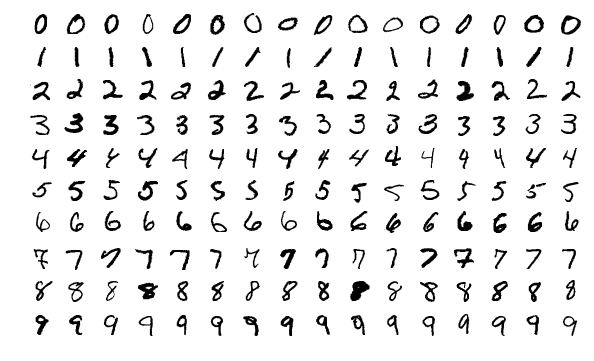
\includegraphics[scale=0.5]{MnistExamples.png}
 % MnistExamples.png: 594x361 px, 72dpi, 20.96x12.74 cm, bb=0 0 594 361
 \caption{Example of MNIST's handwitten digits}
\end{figure}
\subsubsection{Prototype}
My first task is to realise a Sparse Coding prototype to compute Sparse Coding on this dataset, using Python. The aim here, is to understand the underlying principles of this method, you can found this prototype in \texttt{Code directory} of this repository as \texttt{SparseCoding.py}. \\
These are some results of this prototype: For time saving I used only 100 digits as input.

\subsubsection{SPAMS}
SPAMS (SPArse Modeling Software) is an optimization toolbox for solving various sparse estimation problems.
\begin{itemize}
 \item Dictionary learning and matrix factorization (NMF, sparse PCA, ...)
 \item Solving sparse decomposition problems with LARS, coordinate descent, OMP, SOMP, proximal methods
 \item Solving structured sparse decomposition problems (l1/l2, l1/linf, sparse group lasso, tree-structured regularization, structured sparsity with overlapping groups,...).
\end{itemize}
It is developed and maintained by Julien Mairal (Inria), and contains sparse estimation methods resulting from collaborations with various people: notably, Francis Bach, Jean Ponce, Guillermo Sapiro, Rodolphe Jenatton and Guillaume Obozinski.\\
You can find my code from Sparse Coding method on MNIST using SPAMS toolbox on my github \texttt{test\_spams.py}.\\
\newpage
\paragraph{Test 1}
In the first test I used 256 atoms, 2 000 iterations and $\lambda$ = 0.015 to learn the dictionary and the sparse coefficients. 
w\begin{figure}[h]
 \centering
 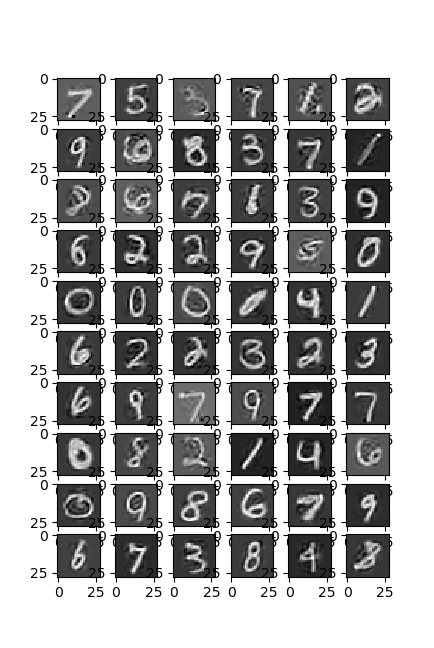
\includegraphics[scale=0.82]{Results/SPAMS_X_ALL_K256/D.png}
 % D.png: 434x648 px, 100dpi, 11.02x16.46 cm, bb=0 0 312 467
 \caption{Few atoms of D}
\end{figure}

 \begin{figure}[h]
 \begin{subfigure}{.5\textwidth}
 \centering
 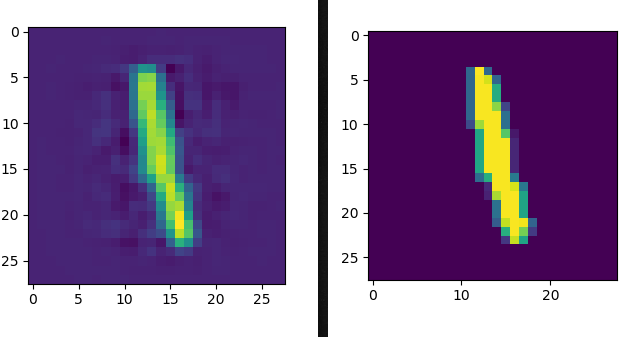
\includegraphics[scale=0.35]{Results/SPAMS_X_ALL_K256/recons_1.png}
  \caption{Reconstructed 1 vs Original 1}
 % module-capteur-laser.jpg: 600x600 px, 72dpi, 21.17x21.17 cm, bb=0 0 600 600
 \end{subfigure}%
  \begin{subfigure}{.3\textwidth}
 \centering
 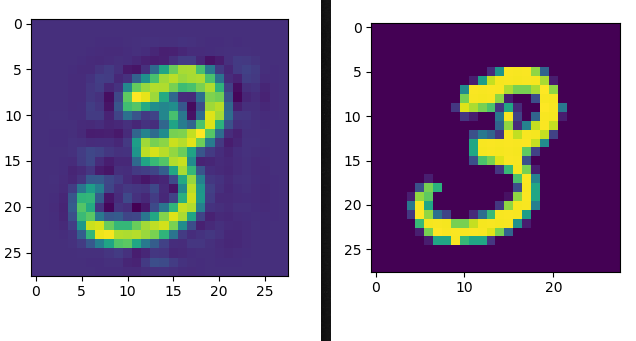
\includegraphics[scale=0.35]{Results/SPAMS_X_ALL_K256/recons_3.png}
 % module-capteur-laser.jpg: 600x600 px, 72dpi, 21.17x21.17 cm, bb=0 0 600 600
  \caption{Reconstructed 3 vs Original 3}

 \end{subfigure}%
\end{figure}

\newpage

\paragraph{Test 2}In the second test I used 1024 atoms, 1 000 iterations and $\lambda = \frac{1.2}{\sqrt{m}}$ \cite{Mairal:2009:ODL:1553374.1553463} \textit{(In my case $\approx 0.0042857$)}.
\begin{figure}[h]
 \centering
 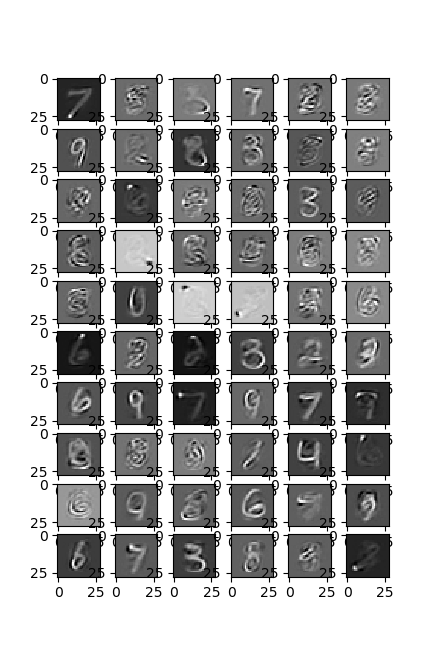
\includegraphics[scale=0.82]{Results/SPAMS_X_ALL_K1024/D.png}
 % D.png: 1873x1022 px, 100dpi, 47.57x25.96 cm, bb=0 0 1349 736
 \caption{Few atoms of D}
\end{figure}
 \begin{figure}[h]
 \begin{subfigure}{.5\textwidth}
 \centering
 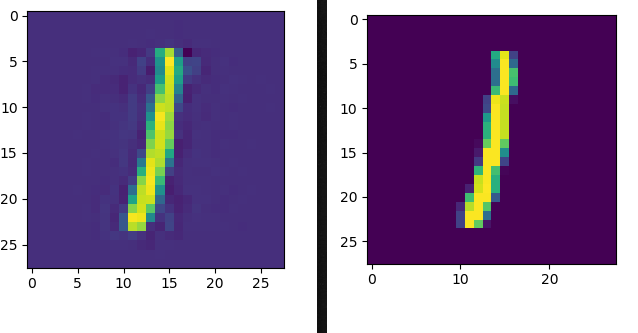
\includegraphics[scale=0.4]{Results/SPAMS_X_ALL_K1024/lambdaopti_recons1.png}
  \caption{Reconstructed 1 vs Original 1}
 % module-capteur-laser.jpg: 600x600 px, 72dpi, 21.17x21.17 cm, bb=0 0 600 600
 \end{subfigure}%
  \begin{subfigure}{.3\textwidth}
 \centering
 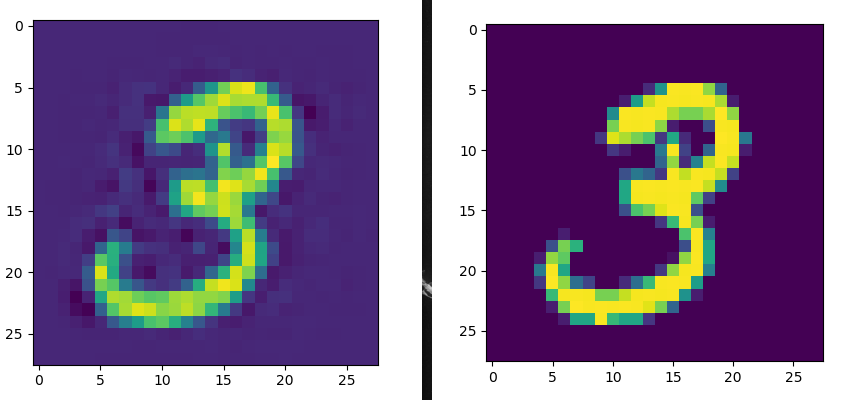
\includegraphics[scale=0.29]{Results/SPAMS_X_ALL_K1024/lambdaopti_recons3.png}
 % module-capteur-laser.jpg: 600x600 px, 72dpi, 21.17x21.17 cm, bb=0 0 600 600
  \caption{Reconstructed 3 vs Original 3}

 \end{subfigure}%
\end{figure}
\newpage
\paragraph{Test 3} In the third test I used 1024 atoms, 1 000 iterations and $\lambda = 5$.
\begin{figure}[h]
 \centering
 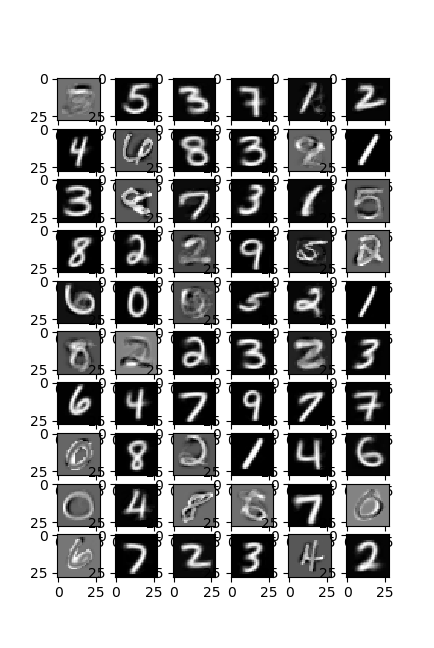
\includegraphics[scale=0.82]{Results/SPAMS_X_ALL_K1024/D_lambdagrand.png}
 % D_lambdagrand.png: 936x994 px, 100dpi, 23.77x25.25 cm, bb=0 0 674 716
 \caption{Few atoms of D}
\end{figure}

 \begin{figure}[h]
 \begin{subfigure}{.5\textwidth}
 \centering
 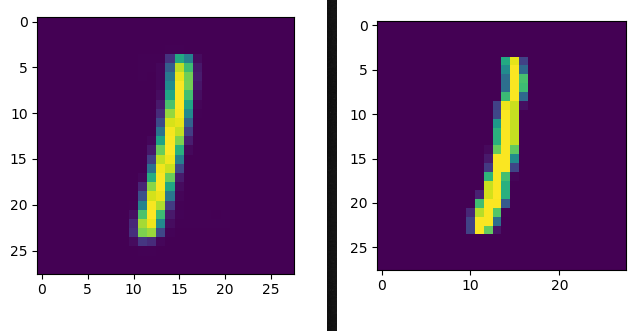
\includegraphics[scale=0.4]{Results/SPAMS_X_ALL_K1024/lambdagrand_recons1.png}
  \caption{Reconstructed 1 vs Original 1}
 % module-capteur-laser.jpg: 600x600 px, 72dpi, 21.17x21.17 cm, bb=0 0 600 600
 \end{subfigure}%
  \begin{subfigure}{.3\textwidth}
 \centering
 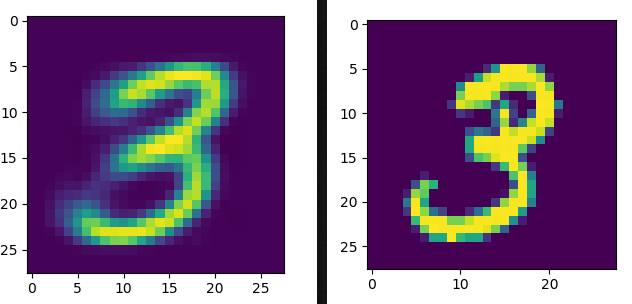
\includegraphics[scale=0.39]{Results/SPAMS_X_ALL_K1024/lambdagrand_recons3.png}
 % module-capteur-laser.jpg: 600x600 px, 72dpi, 21.17x21.17 cm, bb=0 0 600 600
  \caption{Reconstructed 3 vs Original 3}

 \end{subfigure}%
\end{figure}

\newpage
\paragraph{Test 4} In the fourth test I used 2048 atoms, 1 000 iterations and $\lambda = \frac{1.2}{\sqrt{m}}$
\begin{figure}[h]
 \centering
 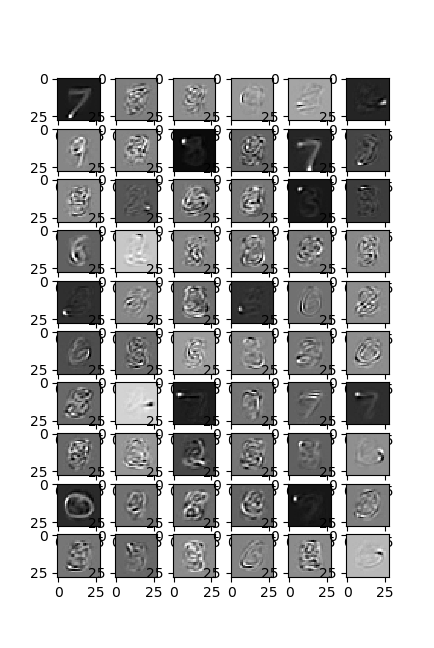
\includegraphics[scale=0.82]{Results/SPAMS_X_ALL_K_2048/D_K2048.png}
 % D_K2048.png: 936x994 px, 100dpi, 23.77x25.25 cm, bb=0 0 674 716
 \caption{Few atoms of D}
 \end{figure}
 
  \begin{figure}[h]
 \begin{subfigure}{.5\textwidth}
 \centering
 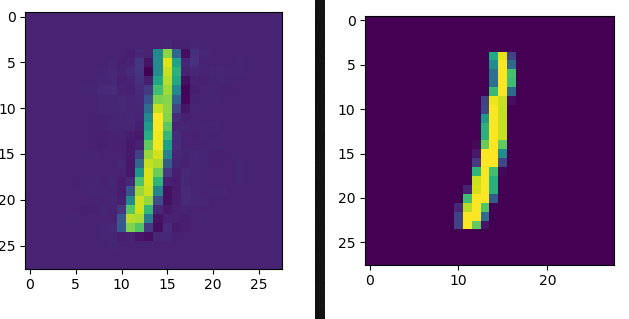
\includegraphics[scale=0.4]{Results/SPAMS_X_ALL_K_2048/recons1.png}
  \caption{Reconstructed 1 vs Original 1}
 % module-capteur-laser.jpg: 600x600 px, 72dpi, 21.17x21.17 cm, bb=0 0 600 600
 \end{subfigure}%
  \begin{subfigure}{.3\textwidth}
 \centering
 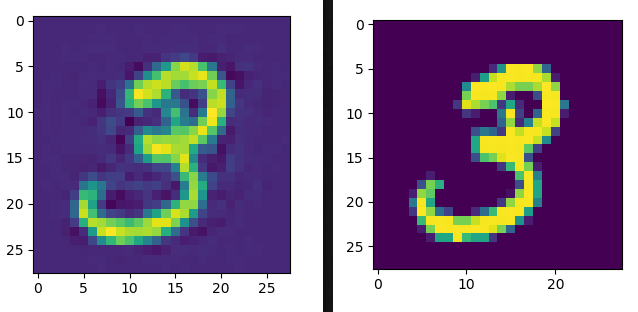
\includegraphics[scale=0.39]{Results/SPAMS_X_ALL_K_2048/recons3.png}
 % module-capteur-laser.jpg: 600x600 px, 72dpi, 21.17x21.17 cm, bb=0 0 600 600
  \caption{Reconstructed 3 vs Original 3}

 \end{subfigure}%
\end{figure}

\newpage
\subsection{Application for Lenna}

\begin{figure}[h]
 \centering
 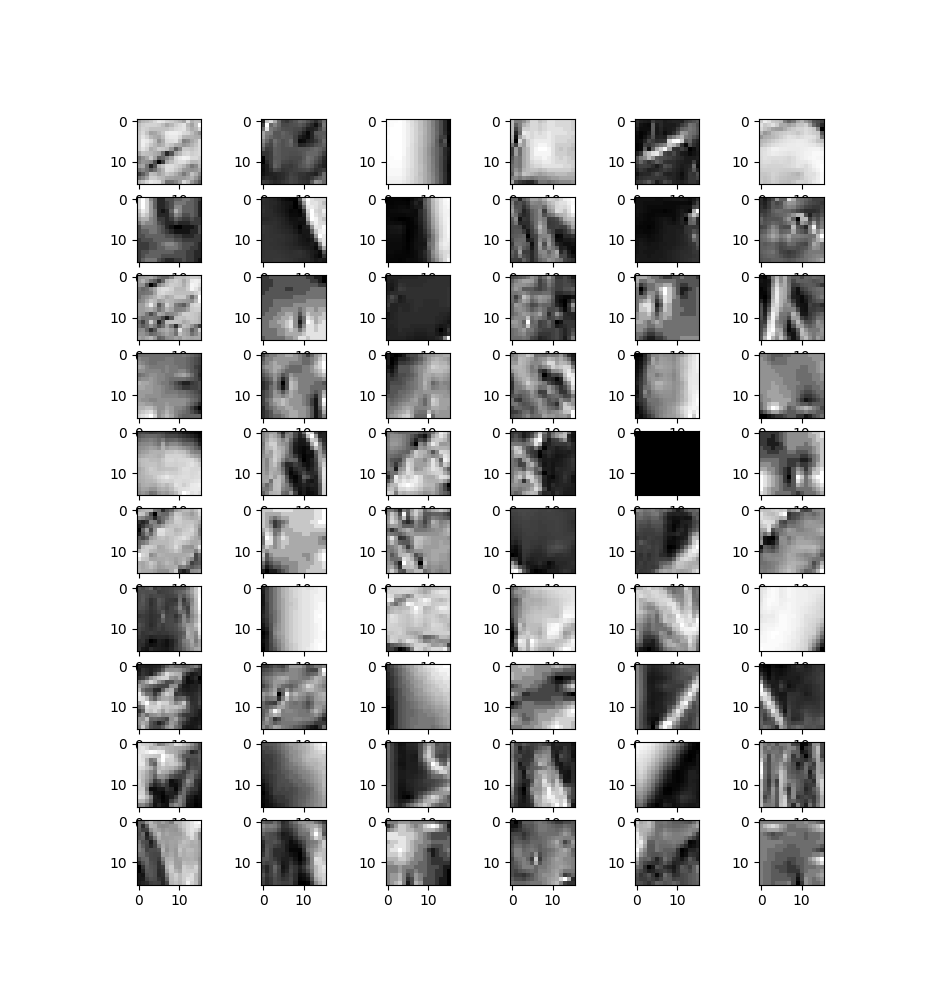
\includegraphics[scale=0.3]{Results/Lenna/lenna_1024.png}
 % lenna_1024.png: 936x994 px, 100dpi, 23.77x25.25 cm, bb=0 0 674 716
 \caption{Some atoms of D when K = 1024}
\end{figure}
\begin{figure}[h]
 \centering
 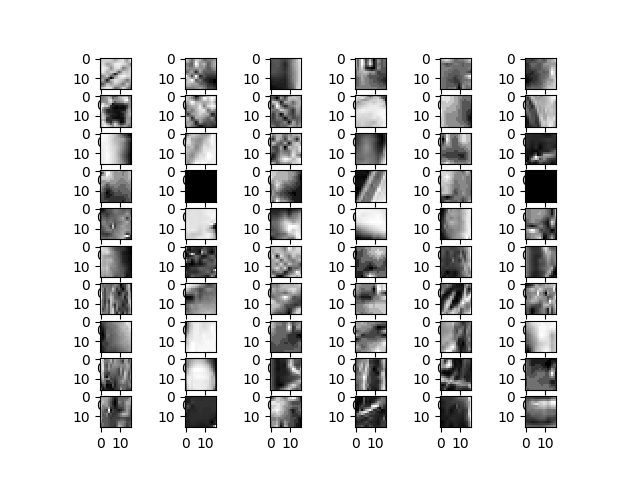
\includegraphics[scale=0.75]{Results/Lenna/lenna_2048.png}
 % lenna_2048.png: 640x480 px, 100dpi, 16.26x12.19 cm, bb=0 0 461 346
 \caption{Some atoms of D when K = 2048}
\end{figure}
\newpage
\subsection{Dictionary learning and sparse coding for unsupervised clustering}
\label{sec:Clustering}
Whereas the previous tests seems have good result, one question appears: \\ \textit{What make us confident about the fact that  two close images (two handwitten 3 for example) have close coefficients representation h ?}\\
Sprechmann and Sapiro \cite{5494985} propose an algorithm to cluster datasets that are well represented in the sparse modeling framework with a set of K learned dictionaries. The main idea is, given a set of K dictionaries, find for each signals the dictionary for which the "best" sparse decomposition is obtainedn, with :

\begin{center}
$\underset{D_i,C_i}{\min} \sum_{i=1}^{K} \sum_{x_j \in C_i} \mathcal{R}(x_j, D_i)$
 
\end{center}
Here $D_i \in \R^{n \times k_i}$ is the $k_i$ dictionary associated with the class $C_i$. $x_j \in \R^n$ are the input data and $\mathcal{R}$  a function that mesure how good the sparse decomposition is for the signal $x_j$ under the dictionary $D_i$. Sprechmann and Sapiro propose to use the cost function in the Lasso-type problem as $\mathcal{R}$ the measure of performance, $\mathcal{R}(x,D) = \|x - D\alpha\|^2_2 + \lambda \|\alpha\|_1$. The class $\mathcal{C}$ for a given signal x is found by solving $\mathcal{C}= \underset{j=1,..,K}{\argmin}$ $ \mathcal{R}(x,Dj) $.

\subsubsection{Dictionary learning for clustering}
Given a set of signals and the number of class, we want to find a set of K learned dictionaries that best represent x (the input data). \cite{5494985} formulate tgus as an energy minimization problemand use the measure previouly proposed,\\
\begin{center}
 $\underset{D_i,C_i}{\min} \sum_{i=1}^{K} \sum_{x_j \in C_i} \underset{\alpha_{ij}}{\min}\|x_j - D_i \alpha_{ij}\|^2_2 + \lambda\|\alpha_{ij}\|_1$
\end{center}
The optimization is carried out by solving one problem at time:
\begin{itemize}
 \item \textit{Assignement step:} The dictionaries are fixed and each signals is assigned to the cluster for which the best representation is obtained.
 \item \textit{Update step:} The new dictionaries are computed fixing the assignation found in the previous step.
\end{itemize}
One drawback of this algorithm is there is no guarantee of reach a global minimum. In this setting, repeated initialization are computationally expensive, thus we need a good initialization.

\subsubsection{Initialization}
The initialization can be given by a set of K dictionaries or as an initial partition of the data.\\
The main idea is to construct a similarity matrix and use it as the input for  a spectral clustering algorithm. Let define $A = [\alpha_1,....,  \alpha_m]$ with $\alpha_j$ the sparse representation of each signal $x_j$. To obtain a good classification, we expect two signal to the same cluster to have decomposition that use similar atoms. Thus we can compute two similarity matrix:
\begin{itemize}
 \item \textit{Clustering the signals :} Construct a similarity matrix $S_1 \in \R^{m \times m}$ which measure the similarity of two signals by comparing the corresponding sparse representation:\\
 $S_1 = |A|^T |A|$
 \item \textit{Clustering the atoms :} Construct a similarity matrix $S_2 \in \R^{k_0 \times k_0}$ ( with $D_0 \in \R^{n \times k_0}$) which represent the similarity of two atoms by comparing how many signals use them simultaneously and how they contribute in their sparse decomposition.\\
 $S_2 = |A||A|^T$
\end{itemize}
In this two case, the similarity matrixes are positive semidefinite and can be associated with a graph: $G_1 = \{X,S_1\}$ and $G_2 = \{D,S_2\}$ where the data (respectivly atoms) are the sets of vertexes with the corresponding $S_i$ as edge weights matrixes. This graph is partitioned using standard spectral clustering algorithm to obtain the initialization.\\
However, when K is large (the number of class), the performance of initial clusterization decreases. To fix this problem \cite{5494985} proposed to stat with the whole set as the only partition and at each itation we subdivise in two sets each of the current partitions, the procedure stops when the desired number of clusters is reached.

\newpage
\section{Discriminative Dictionary }
There are serveral approach for discriminative Dictionary Learning enumerate by \cite{8294264}:
\begin{itemize}
 \item In presence of label:
    \begin{enumerate}
     \item Learn one dictionary per class
     \item Prune large dictionaries
     \item Jointly learn dictionary and classifier
     \item Embed class label into the learning of sparse coefficients
     \item Learn a histogram of dictionary element over signal constituents
    \end{enumerate}

 \item For weakly supervised:\\
    Serveral max margin based, non-convolutive, syntgesis dictionary learning approaches.
\end{itemize}
However in our problem of extract new features for speech we must compare each $\alpha$ with other, thus we must use only one dictionary.
\subsection{One dictionary per class}
The idea is to extend proposed method in  section \ref{sec:Clustering} by adding a term $\mathcal{Q}(D_i,D_j)$ that promotes incoherence between the differents dictionaries, e.g. this term encourage dictionaries to  be independent as possible :
\begin{center}
 $\underset{D_i, C_i}{\min} \sum_{i=1}^{K} \sum_{x_j \in C_i} \mathcal{R}(x_j,D_i) + \eta \sum_{i \neq j} \mathcal{Q}(D_i,D_j)$
\end{center}
For example we can take $\mathcal{Q}(D_i,D_j) = \|D^T_iD_j\|^2_F $ with F denotes Frobenius norm.

\subsection{Supervised Dictionary learning}
\subsubsection{Problem formulation}
In \cite{mairal:inria-00322431} the signal may belong to any of $p$ diffrent classes and they model the signal using a single shared D. The create a set of $p$ decision functions $g_i(x,\alpha,\theta)$ (i = 1,...,p). Where: \\
\begin{center}
  $g_i(x,\alpha,\theta) =     \left\{
                \begin{array}{ll}
                 gi > 0 $ if $x \in $class i $\\
                g_i \leq 0$ otherwise$\\
                \end{array}
              \right.$
\end{center}
The vector $\theta$ parametrizes the model and will be jointly learned with the dictionary D. There are two kinds of models in this paper:\\
\begin{itemize}
 \item \underbar{Linear in $\alpha$:} $g_i(x,\alpha,\theta) = w_i^T \alpha + b_i $ where $ \theta = \{ w_i \in \R^k, b_i \in \R\}_{i=1}^p$
 \item \underbar{Bilinear in $x$ and $\alpha$: }$g_i(x,\alpha,\theta) = x^T W_i \alpha + b_i$ where $ \theta = \{W_i \in \R^{n \times k}, b_i \in \R\}_{i=1}^p$ 
\end{itemize}
They define a \textit{softmax} discriminative cost function as :
\begin{center}
 $\mathcal{C}_i(x_1,..., x_p) = log(\sum_{i=1}^p e^{x_j - x_i})$
\end{center}
Given x, a input signal, with $D$ and $\theta$ fixed, the supervised sparse coding problem for the class $p$ can be computing by :
\begin{center}
 $S^*_i(x,D,\theta) = \underset{\alpha}{\min}S_i(\alpha,x,D,\theta)$
\end{center}
where
\begin{center}
 $S_i(\alpha,x,D,\theta) = \mathcal{C}_i(\{g_j(x,\alpha,\theta)\}^p_{j=1}) + \lambda_0 \|x - D\alpha\|^2_2 + \lambda_1 \|\alpha\|_1$
\end{center}
Then, the classification problem can be compute by: 
\begin{center}
 
$i^*(x,D,\theta) = \underset{i=1,...,p}{\argmin}S^*_i(x,D,\theta)$
\end{center}

\subsubsection{Learning $D$ and $\theta$}
The most direct method for learning $D$ and $\theta$ is to minimize with respect to these (with $T_i$ a sample of input signals corresponding to the class i):
\begin{center}
 $\underset{D,\theta}{\min}(\sum_{i=1}^p \sum_{j \in T_i}S^*_i(x_j,D,\theta))+ \lambda_2 \|\theta\|^2_2$
\end{center}
With  $ \|\theta\|^2_2$ to prevent overfitting. They reffer to this model as SDL-G (Supervised Dictionary Learning - Generative) \cite{mairal:inria-00322431}.\\
A more discriminative approach is not only make $S^*_i$ small for signals with label i but also make the value of $S^*_j$ (with $i \neq j)$ greater than $S^*_i$. To do that they use the softmax cost function $\mathcal{C}_i$:
\begin{center}
  $\underset{D,\theta}{\min}(\sum_{i=1}^p \sum_{j \in T_i} \mathcal{C}_i(\{ S^*_l(x_j,D,\theta)\}^{p}_{l=1}))+ \lambda_2 \|\theta\|^2_2$
\end{center}
But this more difficult to solve, thus they adopt a mixed formulation with SDL-G :
\begin{center}
   $\underset{D,\theta}{\min}(\sum_{i=1}^p \sum_{j \in T_i} \mu \mathcal{C}_i(\{ S^*_l(x_j,D,\theta)\}^{p}_{l=1}) + (1-\mu)S^*_i(x_j,D,\theta))+ \lambda_2 \|\theta\|^2_2$
\end{center}
They refer to this model as SDL-D (Supervised Dictionary Learning - Discriminative). With $\mu$ which control the trade-ff between reconstruction and discrimination.

\subsubsection{Optimization  procedure}
\paragraph{SDL-G}
When $\mu = 0$ or directly SDL-G have the same properties than classical dictionary learning techniques: Using block coordinate descent  consist of iterating between \textit{supervised sparse coding}, where $D$ and $\theta$ are fixed and optimize $\alpha$, and \textit{supervised dictionary update}, where  $\alpha$ is fixed but $D$ and $\theta$ are updated.
\paragraph{SDL-D} However the discriminative version of SDL (where $\mu \neq 0$) is not convex (even when $D$ and $\theta$ or $\alpha$ are fixed). To reach a local minimum for this problem, they have chosen a continuation method: Starting from the generative case and ending with the discriminative one.
\begin{figure}[h]
 \centering
 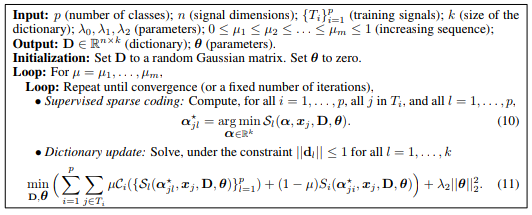
\includegraphics[scale=0.9]{SDL-D.png}
 % SDL-D.png: 532x215 px, 96dpi, 14.07x5.69 cm, bb=0 0 399 161
 \caption{SDL: Supervised dictionary learning Algorithm  \cite{mairal:inria-00322431}}
\end{figure}


\newpage 
\section{Convolutional Sparse Coding}
Notations:
\begin{itemize}
 \item Matrix: Uppercase  \textbf{A}
 \item Vector: Lower-case  \textbf{a}
 \item Scalar: Lower-case a
 \item 2D convolution operation : *
 \item $D \times D$ identity matrix: \textbf{$I_D$}
 \item Kronecker product : $\odot$
 \item $D \times D$ Fourier matrix : \textbf{F}
 \item Hadamard product: $\otimes$
 \item inverse FFT : $ \mathcal{F}^{-1}$
 \item Mapping function that preserve only $M \ll D$ active values relating to the small spaital structure of the estimated filter : $ \mathcal{M}\{\}$
\end{itemize}
\subsection{Idea}
There are other algorithms like Efficient Shift-Invariant Dictionary learning which refers to the problem of discovering a set of latent basis vectors that capture informative \textit{local patterns} at different locations of the input sequences and not in all input sequences \cite{Zheng:2016:ESD:2939672.2939824}, to do that, we will use Convolutional Sparse Coding method.  
\subsection{Problem formulation}
Instead  of decomposing a signal as the $x = Dh$, Convolutional Sparse Coding (CSC) is the summation of convolutions between the feature map and the corresponding filter.
\begin{center}
 $X = \sum_{i=1}^{m} d_i * Z_i$\\  \vspace{0.4cm}
  $\underset{d, z}{\argmin}  \frac{1}{2} \| x - \sum_{k=1}^{K} d_k * z_k \|_2^2 + \beta \|z_k \|_1$\\

\end{center}
This new approach assume the ensemble of input vectors X are independent of one another. But the complexity of convergence is dramatically increase.
Bristow propose an Augmented Lagrangian and the used of  Alternative Direction Method of Multipliers (ADMM) \cite{6618901} to solve this problem. His approach is based on three key points:
\begin{itemize}
 \item The use of ADMM
 \item The convolution subproblem can be solved efficiently (and explicitly) in the Fourier domain (instead of temporal domain)
\item The use of quad-decomposition of the objective into four subproblems (that are convex)
\end{itemize}
In this approach, to solve a Convolutional Sparse Coding problem we introduce two auxilliary variables: \textbf{t} and \textbf{s} and posing the objective in the Fourier domain:
\begin{center}
$\underset{d, s, z, t}{\argmin} \hspace{0.4cm} \frac{1}{2D} \| \hat{x} - \sum_{k=1}^{K} \hat{d}_{k} \odot \hat{z}_k \|^2_2 + \beta \sum_{k=1}^{K} \|t_k\|_1$\\
subject to $\hspace{0.4cm} \|s_k\|^2_2 \leq 1 $ for k = 1.. K\\
                $ \hspace{2.4cm}s_k = \Phi^T \hat{d}_k$ for k = 1..K\\
                $\hspace{1.9cm}z_k = t_k$ for k = 1..K
\end{center}
With $\Phi$ a D $\times$ M submatrix of the Fourier matrix $F = [\Phi,\Phi_\bot]$. In this formulation $\hat{d}_k$ is a D dimensional vector whereas in the original formulation $d_k \in \R^M$  is of a significantly smaller dimensionality to $M \ll D$  corresponding to its smaller spatial support. 
\subsection{Solve the minimization problem}
\subsubsection{Augmented Lagrangian}
We handle the introduction of new equality constraints through an augmented Lagrangian approach \cite{6618901}:\\
\begin{center}
$ \hspace{-8cm} \mathcal{L}(d,s,z,t, \lambda_s, \lambda_t) =$ \\

$ \frac{1}{2D} \| \hat{x} - \sum_{k=1}^{K} \hat{d}_k \odot \hat{z}_k \|^2_2 + \beta \|t\|_1$\\
$ + \lambda^{T}_s(s-[\Phi^T \otimes I_K]\hat{d}) + \lambda^{T}_t (z - t)$\\
$ \hspace{-1.7cm}+ \frac{\mu_s}{2} \| s - [\Phi^T \otimes I_K]\hat{d}\|^2_2$\\
$ \hspace{-3.2cm}+ \frac{\mu_s}{2} \|z-t\|^2_2$
\end{center}
\subsubsection{Quad-decomposion of the objective}
We decompose our objective into four convex subproblems:


\paragraph{Subproblem z}:\vspace{0.5cm}\\
$z^* = \underset{z}{\argmin}$ $\mathcal{L}(z,d,s,t, \lambda_s, \lambda_t)$\\
$ = \mathcal{F}^{-1}\{\underset{z}{\argmin} \frac{1}{2}\|\hat{x} - \hat{D} \hat{z}\| + \hat{\lambda}_t^T(\hat{z}  - \hat{t}) + \frac{\mu_t}{2}\|\hat{z} - \hat{t}\|^2_2\}$\\
$= \mathcal{F}^{-1}\{(\hat{D}^T \hat{D} + \mu_tI)^{-1}(\hat{D}^T \hat{x} +  \mu \hat{t} - \hat{\lambda}_t)\} \vspace{0.6cm}$\\
Where $\hat{D} = [diag(\hat{d}_1),...,diag(\hat{d}_K)]$


\paragraph{Subproblem t}:\vspace{0.5cm}\\
$t^* =  \underset{t}{\argmin}$ $ \mathcal{L}(t,d,s,z,\lambda_s,\lambda_t)$\\
$ =  \underset{t}{\argmin}\frac{\mu_t}{2} \|z - t\|^2_2 + \lambda_t^T(z-t) + \beta\|t\|_1$\\
Unlike subproblem z, the solution to t cannot be efficiently computed in the Fourier domain (since $L_1$ norm is not rotaiton invariant). Solving t requires projecting $\hat{z}$ and $\hat{\lambda}_t$ back into the spatial domain. If this equation does not contain any rotations of the data, each element of t can be solved independently:\vspace{0.3cm}\\
$t^* =  \underset{t}{\argmin} \beta |t| + \lambda_t(z-t) + \frac{\mu}{2}(z-t)^2$\\
Where the optimal value of each t can be found using shrinkage function:\vspace{0.5cm}\\
$t^* = sign(z + \frac{\lambda_t}{\mu_t}) . max\{|z + \frac{\lambda_t}{\mu_t} | - t , 0\}$

\paragraph{Subproblem d}:\vspace{0.5cm}\\
$d^* =  \underset{s}{\argmin}$ $  \mathcal{L}(d,s,z,t,\lambda_s, \lambda_t)$\\ 
$ = \mathcal{F}^{-1} \{ \underset{\hat{d}}{\argmin}\frac{1}{2} \|\hat{x} - \hat{Z}\hat{d}\|^2_2 + \hat{\lambda}_s^T(\hat{d}- \hat{s}) + \frac{\mu}{2}\|\hat{d} - \hat{s}\|^2_2\}$\\
$ = \mathcal{F}^{-1}\{(\hat{Z}^T \hat{Z} + \mu_s I)^{-1} (\hat{Z}^T \hat{x} + \mu_s \hat{s} - \hat{\lambda}_s)\}$
\paragraph{Subproblem s}:\vspace{0.5cm}\\
$s^* =\underset{s}{\argmin}$ $  \mathcal{L}(d,s,z,t,\lambda_s, \lambda_t) $\\
$  = \underset{s}{\argmin}$ $\frac{\mu_s}{2} \|\hat{d} - [\Phi^T \otimes I_K]s\|^2_2 + \hat{\lambda}_s^T(\hat{d} - [\Phi^T \otimes I_K]s)$\\
Solving this equation as it is a quadratically constrained quadratic programming problem (QCQP).  Due to the Kronecker product with the identity matrix $I_K$ it can be broken down into K independent problems:\\
$s^*_k = \underset{s_k}{\argmin}$ $\frac{\mu_s}{2} \|\hat{d}_k  - \Phi^T s_k\|^2_2 + \hat{\lambda}_{sk}^T(\hat{d}_k - \Phi^T s_k)$\\
Futher, since $\Phi$ is orthonormal projectiong the optimal solution to the unconstrained problem cab be found efficiently through:\\

\begin{center}
  $s^* =     \left\{
                \begin{array}{ll}
                 \|\tilde{s}\|^{-1}_2 \tilde{s}_k $ , if $ \|\tilde{s}\|^{-1}_2 \geq 1\\
                \tilde{s}_k $ otherwise$\\
                \end{array}
              \right.$
\end{center}
where,
\begin{center}
 $\tilde{s}_k = (\mu_s \Phi \Phi^T)^{-1} (\Phi \hat{d}_k + \Phi \hat{\lambda}_{sk})$
\end{center}

Finally the solution to this equation can be found using :\\
$\tilde{s}_k = \mathcal{M}\{\frac{1}{\mu_s} \sqrt{D}^{-1}(  \mathcal{F}^{-1}\{\hat{d}_k\} +  \mathcal{F}^{-1}\{\hat{\lambda}_{sk}\}  ) \}$\\


\subsubsection{Lagrange Multiplier Update}
\begin{center}
 $\lambda^{(i+1)}_{t} \leftarrow \lambda^{(i)}_{t}  + \mu_t(z^{(i+1) - t^{(i+1)}}) $\\
 $\lambda^{(i+1)}_{s} \leftarrow \lambda^{(i+1)}_{s}  +\mu_s(d^{(i+1) - s^{(i+1)}}) $\\
\end{center}

\subsubsection{Penalty update}
Convergence may be reach if $\mu^{(i)} \rightarrow \infty$:

\begin{center}
  $\mu^{(i+1)} =     \left\{
                \begin{array}{ll}
                 \tau \mu^{(i)}$ if $\mu^{(i)} < \mu_{max} \\
                \mu^{(i)}$ otherwise$\\
                \end{array}
              \right.$
\end{center}

%====================PART 2 SPARSE CODING FOR SR=========
\newpage
\section{Sparse Coding for speech recognition}
In this part of the paper we will see novel feature exraction technique based on the principles of sparse coding \cite{DL_speech_reco}. Sparse codigin deals with the problem of how represent a given audio input as a linear combination of a minimum number of basis function. The weights of the linear combination are used as feature for speech recognition (acoustic modeling). Note the input dimensionality is typically \textbf{much} less than the number of atoms in the dictionary \textit{i.e.} we use overcomplete dictionary.\\
We use Sparse Coding algorithm as describe before and we get the dictionary D and  the matrix of sparse coefficients  h.\\
\paragraph{Reflection path} In \cite{DL_speech_reco} they used spectro-temporal speech domain wich is obtained by performing a short time Fourier transform (STFT) with an analysis window of length 25 ms and a frameshit of 10 ms on the input signal. Log critical band energies are subsequently obtained by projecting the magnitude square values of the STFT output on a set of frequency weights, which are equally spaced on the Bark frequence scale, and then applying a logarithm on the output projections.
\newpage
\bibliographystyle{plain}
\bibliography{efficient-sparse-coding-algorithms.bib}

\end{document}
%KSVD
%OMP
% k doit etre deux fois trois plus grand que 8x8
%sapiro Author 
